\documentclass{article}

% Language setting
% Replace `english' with e.g. `spanish' to change the document language
\usepackage[spanish]{babel}

% Set page size and margins
% Replace `letterpaper' with `a4paper' for UK/EU standard size
\usepackage[letterpaper,top=2cm,bottom=2cm,left=3cm,right=3cm,marginparwidth=1.75cm]{geometry}

% Useful packages
\usepackage{amsmath}
\usepackage{graphicx}
\usepackage[colorlinks=true, allcolors=blue]{hyperref}

\title{Lineas de Balmer}
\author{César de la Rosa Sobrino}

\begin{document}
\maketitle

\renewcommand{\abstractname}{Resumen}
 
\begin{abstract}
Comprobamos experimentalmente las longitudes de onda de lineas de emision del hidrógeno en el espectro visible. Para ello utilizamos una lámpara de Balmer cuya luz se descompone con una red de difracción y se proyecta en una pantalla milimetrada. Con varias medidas comprobamos que a cada longitud de onda le corresponde un ángulo de difracción y los medimos. Finalmente también calculamos la constante de Rydberg ($R_H$) en base a los resultados experimentales.
\end{abstract}

\section{Introducción}
-Espectros de emisión por excitación de los electrones (cambio del nivel de energía) \\
-Lineas de Balmer\\
-Constante de Rydberg y frecuencia de Rydberg.\\
-Difracción de la luz en la red de difracción\\

\section{Procedimiento experimental}
En nuestro montaje experimental, gracias al cual buscaremos comprobar las descripciones teóricas, contamos con una  lámpara de Balmer, dos lentes convergentes, una rendija ajustable, una red de difracción de Rowland, una pantalla translúcida milimetrada y un carril guía en el que situamos nuestros instrumentos y determinamos su posicion.
La lámpara del Balmer contiene vapor de agua que mediante descargas eléctricas se divide en hidrógeno e hidroxilo. El hidrógeno, al ser excitado emite fotones en las longitudes de onda correspondientes a los saltos de niveles de energía que dan sus electrones. Esta luz pasa a una lente de distancia focall $f = 50 mm$ que hace converger la luz en una rendija de apertura regulable. La luz incide entonces sobre otra lente de distancia focal $f = 100 mm$ de forma que se enfoca nítidamente en la pantalla. Si no colocamos nuestra red de difraccción, aparece una linea blanca en el centro de la pantalla, sim embargo, al colocar la rendija entre la lente y la pantalla, aparecen además las lineas de difracción de orden uno en distintas posiciones según su longitud de onda y simétricamente a izquierda y derecha. Comprobamos así mismo, que al acercar nuestra red de difracción a la pantalla las lineas se acercan a la linea de orden cero (e incluso somos capaces de ver alguna linea de orden dos) mientras que si la alejamos las lineas se alejan. Lo que se mantiene constante es el ángulo de difracción.\\
Para ser capaces de medir el ángulo de difracción, tomaremos repetidas medidas las posiciones de las lineas del Balmer en la pantalla variando la posición de la red de dispersión. De esta manera, conociendo las características de la 
\section{Resultados}

\begin{figure}[h]
    \begin{minipage}{0.6\textwidth}
        \centering
        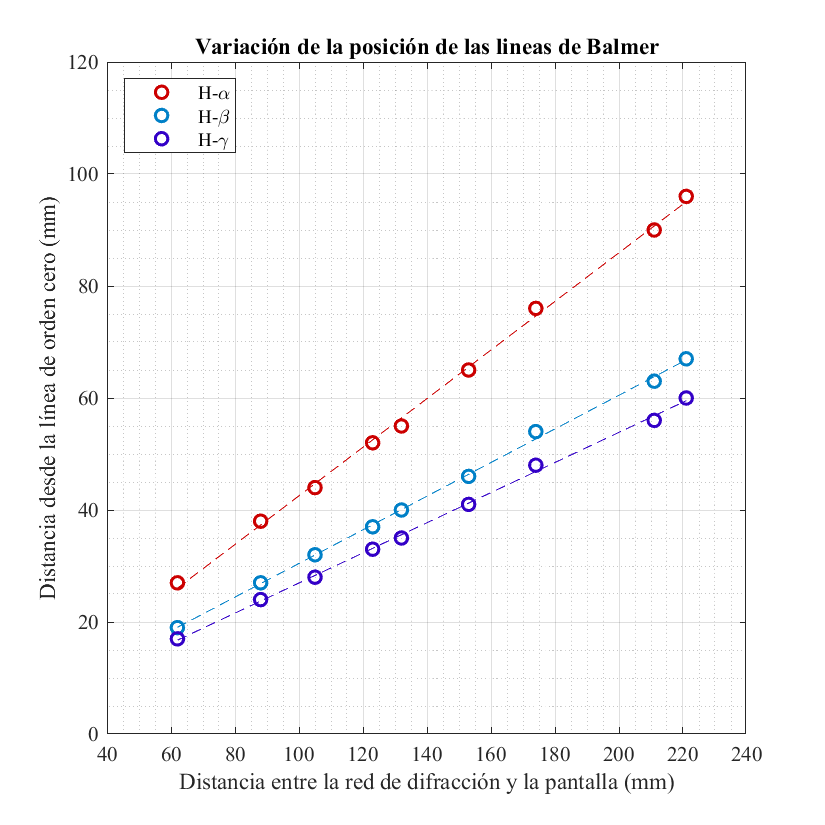
\includegraphics[width=\linewidth]{Lineas_de_Balmer.png}
        \caption{Descripción del gráfico.}
        \label{fig:nombre_del_archivo}
    \end{minipage}\hfill
    \begin{minipage}{0.4\textwidth}
        \centering
        \begin{tabular}{c|ccc}
         $a$ ($mm$)& $b_{H-\alpha}$ ($mm$) & $b_{H-\beta}$ ($mm$) & $b_{H-\gamma}$ ($mm$)\\ \hline
         62 $\pm$ 1& 27  $\pm$ 1& 19  $\pm$ 1& 17 $\pm$ 1\\
         88 $\pm$ 1& 38 $\pm$ 1& 27  $\pm$ 1& 24 $\pm$ 1\\
         91 $\pm$ 1&  41 $\pm$ 1&29   $\pm$ 1&26  $\pm$ 1\\
         105 $\pm$ 1&  44 $\pm$ 1& 32  $\pm$ 1&28 $\pm$ 1 \\
         123 $\pm$ 1&  52 $\pm$ 1& 37 $\pm$ 1 & 33 $\pm$ 1\\
         132 $\pm$ 1&  55 $\pm$ 1& 40 $\pm$ 1 & 35 $\pm$ 1\\
         153 $\pm$ 1&  65 $\pm$ 1& 46 $\pm$ 1 & 41 $\pm$ 1\\
         174 $\pm$ 1&  76 $\pm$ 1& 54 $\pm$ 1 & 48 $\pm$ 1\\
         211 $\pm$ 1&  90 $\pm$ 1& 63  $\pm$ 1& 56 $\pm$ 1\\
         221 $\pm$ 1&  96 $\pm$ 1& 67 $\pm$ 1 & 60 $\pm$ 1\\
    \end{tabular}
    \caption{Distancia entre las líneas de Balmer y la línea de orden cero en función de la distancia red-pantalla}
    \label{tab:my_label}
    \end{minipage}
\end{figure}
\section{Análisis de resultados}
Nuestro trabajo en el laboratorio nos ha permitido medir las longitudes de onda de las lineas de emisión del hidrógeno en el espectro visible con una incertidumbre baja. Además, al comparar los resultados obtenidos con los resultados reales de esas longitudes de onda, comprobamos que los mismos se encuentran en nuestro intervalo de incertidumbre con lo que podemos decir que nuestro error ha sido también mínimo:
(TABLA)
Así mismo, podemos calcular cual sería nuestra constante de Rydberg experimental apoyándonos en la fórmula (). Tras comparar los resultados obtenidos con el real, podemos comprobar que los mismos se adecuan a la formula descrita por Rydberg que sería una de las primeras comprobaciones experimentales de la historia del comportamiento cuántico de los átomos:
(TABLA)
\section{Conclusiones}
Tras analizar los resultados obtenidos y compararlos con los de la literatura, podemos concluir que hemos comprobado experimentalmente la descripción teórica de las lineas de emisión del hidrógeno.
\bibliographystyle{alpha}
\bibliography{sample}

\section{Anexo}

\end{document}